\documentclass[notes2924]{subfiles}
\begin{document}
	\setcounter{chapter}{9}
	\chapter{Parametric Equations and Polar Coordinates}
	\addcontentsline{toc}{section}{10.1 - Curves Defined by Parametric Equations }
	\setcounter{section}{1}
	\setcounter{ex}{0}
	\fancyhead[RO,LE]{\bfseries \large\nameref{cs101}} 
	\fancyhead[LO,RE]{\bfseries \currentname}
	\fancyfoot[C]{{}}
	\fancyfoot[RO,LE]{\large \thepage}	%Footer on Right \thepage is pagenumber
	\fancyfoot[LO,RE]{\large Chapter 10.1}
	
\section*{Curves Defined by Parametric Equations}\label{cs101}
	\subsection*{Before Class}
	\addcontentsline{toc}{subsection}{Before Class}
	\subsection*{Parametric Equations}
	\addcontentsline{toc}{subsubsection}{Parametric Equations}

		\begin{question}
			The picture below does \emph{not} describe a function?  Why?
		\end{question}
		\begin{flushleft}
			\begin{tikzpicture}
  	  			\begin{axis}[
    				axis x line = middle,
    				axis y line = middle,
	    			axis line style = {<->, color=black},
    				every axis y label/.style=
{at={(ticklabel cs:1.1)}},
    				ylabel = {$y$},
    				every axis x label/.style= {at ={(ticklabel cs:1)}},
    				xlabel = {$x$},
					xmin=-4.5,xmax=4.5,
       		    	ymin=-9.5,ymax=4.5,
	       		    xtick = {-4,-2,2,4},
    	   		    ytick = {-8,-6,-4,-2,2,4},
        	    ]
        		    \addplot [domain=-3:3,samples=50]({x^3-3*x},{3*x^2-9}); 
   				 \end{axis}
			\end{tikzpicture}
		\end{flushleft}
		
		\begin{defn}[Parameter/Parametric Equation]
			Let $C$ be a curve, and let the functions $x =f(t)$ and $y = g(t)$ describe the $x-$ and $y-$coordinate of $C$.  The variable $t$ is called the \textbf{parameter}, and the function $x = f(t)$ and $y = g(t)$ are called \textbf{parametric equations}.
		\end{defn}
			\newpage

		\begin{ex}
			Consider the parametric equations $x(t) = t-2$ and $y(t) = t^2 - 2t$.
			\begin{enumerate}[(a)]
				\item Fill out the table below.\\
					\begin{tabular}{|c|P{1.25in}|P{1.25in}|c|P{1.25in}|P{1.25in}|}\hline
						 $t$	&  $x$	&  $y$  & $t$	& $x$	& $y$	\\ \hline
						 		&		&		&		&			&		\\
						 $-2$	&		&		& $2$	&			&		\\
						 		&		&		&		&			&		\\ \hline 
						 		&		&		&		&			&		\\
						 $-1$	&		&		& $3$	&			&		\\
						 		&		&		&		&			&		\\ \hline
						 		&		&		&		&			&		\\
						 $0$	&		&		& $4$	&			&		\\
						 		&		&		&		&			&		\\ \hline
						 		&		&		&		&			&		\\
						 $1$	&		&		&		&			&		\\
						 		&		&		&		&			&		\\  \hline
					\end{tabular}
				\item Plot the points from the table on the graph below.  Connect the plotted points to see the parametric curve, and draw arrows to indicate its direction of travel.  What kind of function do you see?
					\begin{flushleft}
						\begin{tikzpicture}[scale = 1.25]
							\begin{axis}[
							axis x line = middle,
							axis y line = middle,
							axis line style = {<->, color=black},
							xmin = -4.5, xmax = 4.5,
							ymin = -1.5, ymax = 8.5,
							xtick = {-4-3,-2,-1,1,2,3,4},
							ytick = {-1,1,2,3,4,5,6,7,8},
							]
							%\addplot[domain=-4.:4.,smooth,samples=100] {(x+2)^2-2*(x+2)};
							\end{axis}
						\end{tikzpicture}
					\end{flushleft}
			\end{enumerate}
		\end{ex}
			\newpage

		\begin{ex}
			Rather than plotting points, we could have directly seen the function.  We can do this by a process called \emph{eliminating the parameter}.
			\begin{enumerate}[(a)]
				\item Given the parametric equations $x= t-2$ and $y= t^2-2t$, eliminate the parameter to show that the parametric curve is given by the function $y =x^2-2x$
					\vs{1}
					
				\item If we wanted to only include the \emph{right} portion of the graph shown, what sort of restriction would we need to put on $t$?
					\vs{.5}
			\end{enumerate}
		\end{ex}
		
		\begin{ex}
			Eliminate the parameter to find the curve represented by the parametric equations $x = \sqrt{t}$, $y = t^2+1$.  There is a natural restriction on the time interval; what is it?
		\end{ex}
			\vs{1}
		\newpage
		
		\begin{ex}
			$ $
			\begin{enumerate}[(a)]
				\item What curve is represented by the parametric equations $x = \cos t$, $y = \sin t$, $0\leq t\leq 2\pi$?
					\vs{1}
				\item The parametric equations $x = \cos 2t$, $y = \sin 2t$, $0\leq t\leq 2\pi$ represent the same curve as in part (a).  What is the difference between the parametrizations in (a) and (b)?
					\vs{1}
				\item What if in (b) we instead took the time interval $0\leq t\leq \pi$?  What would be the difference between (a) and (b) in that case?
					\vs{1}
			\end{enumerate}
		\end{ex}
			\newpage
			
	\subsection*{Pre-Class Activities}
		\begin{ex}
			Use this space to write any questions you might have from the videos.
		\end{ex}
			\vs{.5}
			
		\begin{ex}
			For each of the following parametric curves, sketch the curve and indicate the direction in which the curve is traced as $t$ increases.  Then, eliminate the parameter to find a Cartesian equation for the curve.
			\begin{enumerate}[(a)]
				\item $x = 2t -1 $, $y = \dfrac{1}{2}t + 1$
					\vs{1}
					
				\item $x = t^2 -3$, $y = t+2$, $-3\leq t\leq 3$
					\vs{1}
					
				\item $x = \sin t$, $y = 1-\cos t$, $0\leq t\leq 2\pi$
					\vs{1}
			\end{enumerate}
		\end{ex}
			\newpage
			
	\subsection*{In Class}
	\subsubsection*{Examples}
		\begin{ex}
			Sketch the curve $x = \sin \lrpar{\dfrac{1}{2}\theta}$, $y = \cos \lrpar{\dfrac{1}{2}\theta}$, $-\pi\leq\theta\leq\pi$.  Then, eliminate the parameter to find a Cartesian expression for the curve.
		\end{ex}
			\vs{1}
			
		\begin{ex}
			Do the same thing for the parametric equations $x = e^t$, $y = e^{-2t}$.
		\end{ex}
			\vs{1}
			
		\begin{ex}
			Describe the motion of a particle with position $x = 5+2\cos (\pi t)$, $y =3 + 2\sin (\pi t)$ as $t$ varies in the interval $[1,2]$.
		\end{ex}		
			\vs{1}
			\newpage
			
		\begin{ex}
			Match the graphs of the parametric equations $x = f(t)$ and $y = g(t)$ in (a)-(d) with the parametric curves labeled I - IV.  Justify your response.\\
			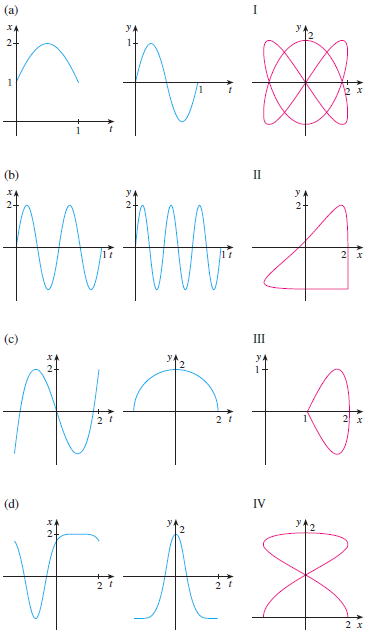
\includegraphics[scale = 1.25]{101_1.png}
		\end{ex}
			\newpage
			
		\begin{ex}
			Develop a parametrization which traces out a circle three times in the time interval $0\leq t \leq \pi$.
		\end{ex}
			\vs{1}
			
		\begin{ex}
			Compare the curves represented by the parametric equations given.  How do they differ?
			\begin{enumerate}[(a)]
				\item $x = t^3$, $y = t^2$
				\item $x = e^{-3t}$, $y =e^{-2t}$
				\item $x = t^6$, $y = t^4$
			\end{enumerate}
		\end{ex}
			\vs{1}
			\newpage
			
	\subsection*{After Class Activities}
		\begin{ex}
			Sketch the parametric curve $x = t^2$, $y = t^3$, and eliminate the parameter to find a Cartesian equation for the curve.
		\end{ex}
			\vs{1}
			
		\begin{ex}
			Do the same thing for the curve $x = t^2$, $y = \ln t$
		\end{ex}
			\vs{1}
			
		\begin{ex}
			Describe the motion of a particle with position $x = 2 + \sin t$, $y = 1 + 3\cos t$ on the interval $\pi/2\leq t\leq 2\pi$.  
		\end{ex}
			\vs{.5}
			\newpage
			
		\begin{ex}
			Compare the curves represented by the parametric equations below.  How do they differ?
			\begin{enumerate}[(a)]
				\item $x = t$, $y = t^{-2}$
				\item $x = \cos t$, $y = \sec t$
				\item $x = e^t$, $y = e^{-2t}$
			\end{enumerate}
		\end{ex}
			\vs{1}
			
		\begin{ex}
			The graphs of $x = f(t)$ and $y = g(t)$ are given below.  Use the graphs to sketch the corresponding parametric curve; use arrows to indicate the direction in which the curve travels.\\
			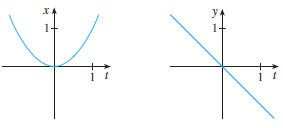
\includegraphics[scale = 1.25]{101_2.png}
		\end{ex}
			\vs{1}
	
\clearpage
\end{document}